\newpage
\section{Auswertung}

\subsection{Einstellen der Diskreminatorschwelle}
Das Einstellen der Diskreminatorschwelle mithilfe des Vielkanalanalysators ergibt die in Tabelle \ref{tab:diskreminatorschwelle} aufgetragenen Messwerte. Es soll erreicht werden, dass sich die Zählrate von $0\,\symup{mbar}$ auf
$1000\,\symup{mbar}$ mindestens halbiert. Unter den jeweiligen Einstellungen des Vielkanalanalysators können die weiteren Versuchsteile durchgeführt werden.


\begin{table}[htbp]
\centering
\caption{Messwerte beim Einstellen der Diskreminatorschwelle.}
\label{tab:diskreminatorschwelle}
\begin{tabular}{S[table-format=1.1] S[table-format=4] S[table-format=3] S S[table-format=5] }
\toprule
{$l/ \,10^{-2}\symup{m}$} & {$p/10^{-3}\, \symup{bar}$} & {$\symup{Counts}$} & {$\symup{Kanal}$} & {Zählrate} \\
\midrule
1.5    & 0      & 457 & 527 & 76537 \\
       & 1000   & 584 & 366 & 33072 \\

\midrule	
2       & 0      & 249 & 366 & 56593\\
        & 1000   & 331 & 527 & 7887 \\


\bottomrule
\end{tabular}
\end{table}






\subsection{Reichweite der {\texorpdfstring{$\alpha$}{Alpha}}-Strahlung}
Zur Berechnung der mittleren Reichweite der $\alpha$-Teilchen werden die Zählraten der jeweiligen eingestellten Abstände $l$ gegen die effektive Länge $x_0$, welche über Gleichung \ref{eq:reichweite} berechnet wird, aufgetragen.
Die verwendeten Messdaten können aus Tabelle \ref{tab:reichweite} entnommen werden. In diesen sind die Drücke $p$, die Counts, die Kanäle und die Zählraten, welche vom Computerprogramm ausgegeben wurden, sowie die effektive Länge $x_0$ und die
entsprechenden Energien $E$ zu finden. Für die letzte Größe wird für $0\,\symup{mbar}$ eine Energie von $4\,\symup{MeV}$ gesetzt, alle weiteren Energien werden proportional über die Kanäle bestimmt.

\begin{table}[h!tbp]
\centering
\caption{Messwerte zur Bestimmung der mittleren Reichweite.}
\label{tab:reichweite}
\begin{tabular}{S[table-format=1.1] S[table-format=4] S[table-format=4] S[table-format=3] S[table-format=6] S[table-format=2.2] S[table-format=1.2] }
\toprule
{$l/ \,\symup{cm}$} & {$p/\, \symup{mbar}$} & {$\symup{Counts}$} & {$\symup{Kanal}$} & {Zählrate} & {$x_0 /\,\symup{mm}$} & {$E /\,\symup{MeV}$} \\
\midrule
1.5    & 0   & 941 & 527 & 161877 & 0 & 4\\
       & 50  & 963 & 495 & 161277 & 0.74 & 3.76 \\
	   & 100 & 950 & 495 & 157732 & 1.48 & 3.76 \\
	   & 150 & 1010 & 483 & 157625 & 2.22 & 3.67 \\	   
	   & 200 & 1065 & 463 & 156034 & 2.96 & 3.51\\
	   & 250 & 1096 & 463 & 153792 & 3.70 & 3.51\\
	   & 300 & 1064 & 463 & 152001 & 4.44 & 3.51\\
	   & 350 & 1102 & 455 & 150500 & 5.18 & 3.45\\
	   & 400 & 1061 & 448 & 147357 & 5.92 & 3.4\\
	   & 450 & 1157 & 431 & 145209 & 6.66 & 3.27\\
	   & 500 & 1159 & 423 & 142490 & 7.40 & 3.21\\
 	   & 550 & 1147 & 419 & 138768 & 8.14 & 3.18\\
	   & 600 & 1180 & 419 & 135112 & 8.88 & 3.18\\
	   & 650 & 1255 & 399 & 131522 & 9.62 & 3.03\\
	   & 700 & 1306 & 399 & 126386 & 10.37 & 3.03\\
	   & 750 & 1404 & 399 & 121800 & 11.11 & 3.03\\
	   & 800 & 1308 & 391 & 115545 & 11.85 & 2.97\\
	   & 850 & 1333 & 367 & 108058 & 12.59 & 2.79\\
	   & 900 & 1360 & 376 & 100227 & 13.33 & 2.85\\
	   & 950 & 1401 & 367 & 98248 & 14.07 & 2.79\\
	   & 1000 & 1355 & 367 & 75984 & 14.81 & 2.79\\
\midrule
2      & 0   & 657 & 515 & 114855 & 0 & 4\\
       & 50  & 672 & 511 & 112216 & 0.99 & 3.97\\
	   & 100 & 681 & 495 & 112152 & 1.97 & 3.84\\
	   & 150 & 682 & 463 & 111337 & 2.96 & 3.59\\	   
	   & 200 & 789 & 463 & 108275 & 3.95 & 3.59\\
	   & 250 & 759 & 455 & 106929 & 4.93 & 3.53\\
	   & 300 & 765 & 463 & 104299 & 5.92 & 3.59\\
	   & 350 & 780 & 448 & 103377 & 6.91 & 3.48\\
	   & 400 & 836 & 431 & 99788 &  7.89 & 3.35\\
	   & 450 & 840 & 415 & 98292 & 8.88 & 3.22\\
	   & 500 & 866 & 399 & 93292 & 9.87 & 3.09\\
 	   & 550 & 879 & 399 & 89007 & 10.86 & 3.09\\
	   & 600 & 893 & 399 & 84418 & 11.85 & 3.09\\
	   & 650 & 949 & 399 & 77557 & 12.83 & 3.09\\
	   & 700 & 932 & 367 & 69840 & 13.82 & 2.85\\
	   & 750 & 944 & 367 & 61664 & 14.81 & 2.85\\
	   & 800 & 965 & 367 & 53202 & 15.79 & 2.85\\
	   & 850 & 929 & 367 & 42037 & 16.78 & 2.85\\
	   & 900 & 793 & 367 & 31698 & 17.77 & 2.85\\
	   & 950 & 663 & 367 & 23749 & 18.76 & 2.85\\
	   & 1000 & 370 & 367 & 12139 & 19.74 & 2.85\\
\bottomrule
\end{tabular}
\end{table}


\begin{figure}[h!tbp]
	\centering
	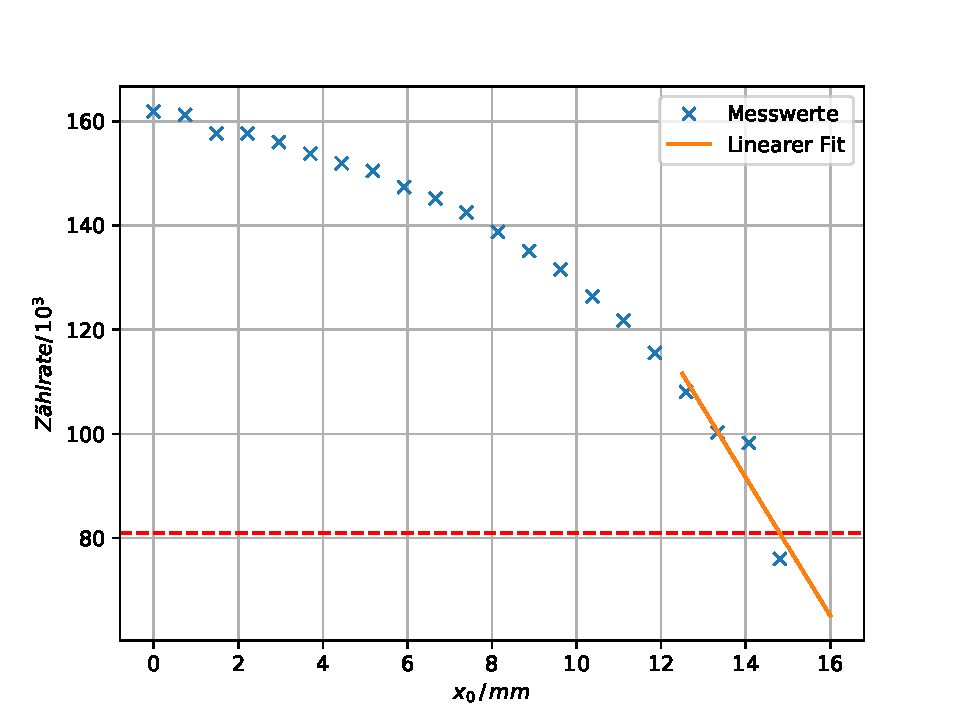
\includegraphics[width=0.8\linewidth]{zaehlrate_weglaenge.pdf}
	\caption{Zählrate als Funktion der effektiven Länge $x_0$ für $l=1{,}5\,\symup{cm}$.}
	\label{fig:zaehlrate1}
\end{figure}

\begin{figure}[h!tbp]
	\centering
	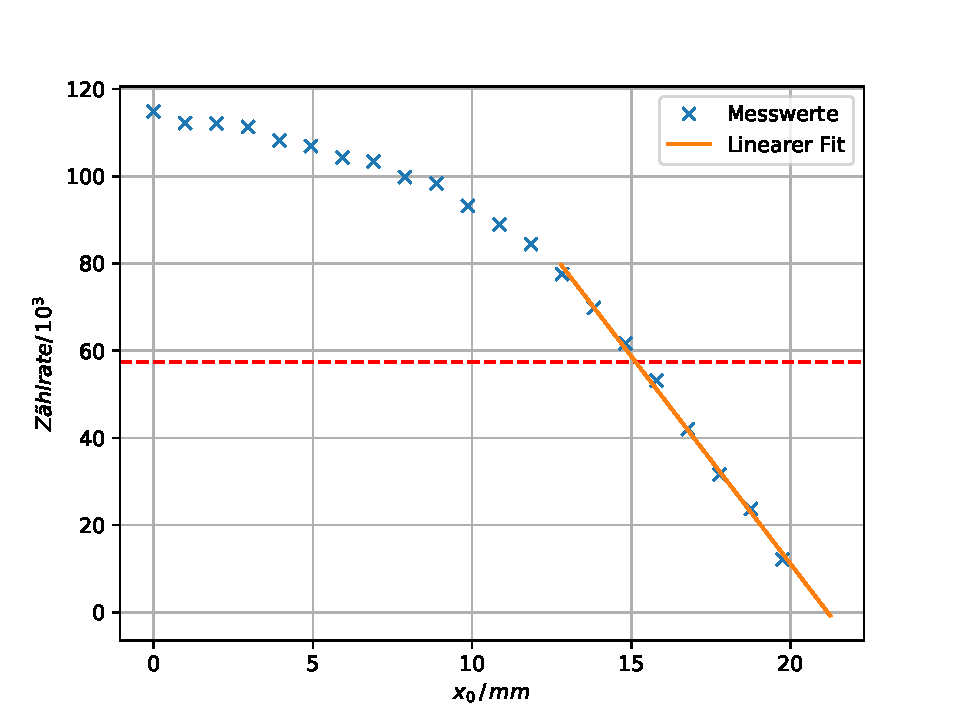
\includegraphics[width=0.8\linewidth]{zaehlrate_weglaenge2.pdf}
	\caption{Zählrate als Funktion der effektiven Länge $x_0$ für $l=2\,\symup{cm}$.}
	\label{fig:zaehlrate2}
\end{figure}



Die Abbildungen \ref{fig:zaehlrate1} und \ref{fig:zaehlrate2} zeigen die Zählraten in Abhängigkeit der effektiven Länge. Auf Höhe der halben maximalen Zählrate $\frac{N_{\text{max}}}{2}$ wird eine Horizontale gelegt. 
Zudem wird mithilfe des Pythonmoduls matplotlib in den annähernd linear abfallenden Bereichen der beiden Funktionen eine lineare Regression der Form

\begin{equation*}
y = mx + b
\end{equation*}
vorgenommen. Es ergeben sich für Steigung und Y-Achsenabschnitt:
\begin{equation*}
\begin{aligned}
l = 1{,}5\,\symup{cm:}\,\, m &= -13{,}3 \pm 3{,}9 \\
                         b &= 277{,}4 \pm 547{,}5 \\
l = 2\,\symup{cm:}\,\,   m &= -9{,}5  \pm 0{,}2\\
                         b &= 201{,}5 \pm 3{,}6 \\ 
\end{aligned}
\end{equation*}


Der Schnittpunkt der beiden eingezeichneten Geraden entspricht der mittleren Reichweite der $\alpha$-Strahlung und kann über

\begin{equation*}
\begin{aligned}
\frac{N_{\text{max}}}{2} &= mx + b \\
x &= \frac{1}{m} \biggl(\frac{N_{\text{max}}}{2} - b \biggr) \\
\end{aligned}
\end{equation*}
berechnet werden. Da es sich bei $m$ und $b$ um fehlerbehaftete Größen handelt, muss auch für $x$ ein Fehler $\Delta x$ berechnet werden. Dies geschieht über die Gaußsche Fehlerfortpflanzung: 

\begin{equation*}
\Delta x = \sqrt{\biggl(-\frac{1}{m^2} \biggl( \frac{N_{\text{max}}}{2} - b \biggr)\biggr)^2 \cdot (\Delta m)^2 + \biggl(\frac{1}{m}\biggr)^2 \cdot (\Delta b)^2}
\end{equation*}

Die mittleren Reichweiten der $\alpha$-Strahlung betragen damit:

\begin{equation*}
\begin{aligned}
x_{1{,}5} &= (0{,}015 \pm 2{,}707\cdot 10^{-7})\,\symup{m}\\
x_{2}  &= (0{,}015 \pm 3{,}789\cdot 10^{-7})\,\symup{m}\\
\end{aligned}
\end{equation*}

Durch Umstellen von Gleichung \ref{eq:reichweiteenergie} und Einsetzen der berechneten mittleren Reichweiten lassen sich die zugehörigen Energie $E_{\text{\alpha}}$ bestimmen.
Es ergibt sich:

\begin{equation*}
\begin{aligned}
E_{\text{1.5}} &= 2{,}86\,\symup{MeV} \\
E_{\text{2}} &= 2{,}86\,\symup{MeV} \\
\end{aligned}
\end{equation*}


In den Abbildungen \ref{fig:energie1} und \ref{fig:energie2} sind die Energien $E$ als Funktion der effektiven Länge zu sehen.

\begin{figure}[h!tbp]
	\centering
	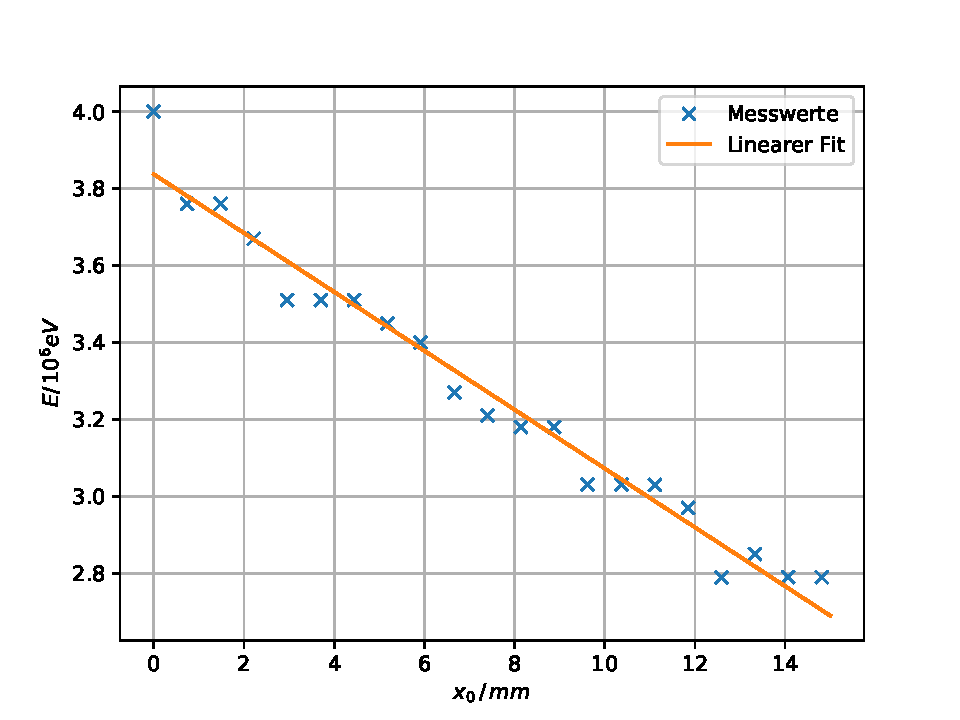
\includegraphics[width=0.8\linewidth]{energie_weglaenge.pdf}
	\caption{Energie als Funktion der effektiven Länge $x_0$ für $l=1{,}5\,\symup{cm}$.}
	\label{fig:energie1}
\end{figure}

\begin{figure}[h!tbp]
	\centering
	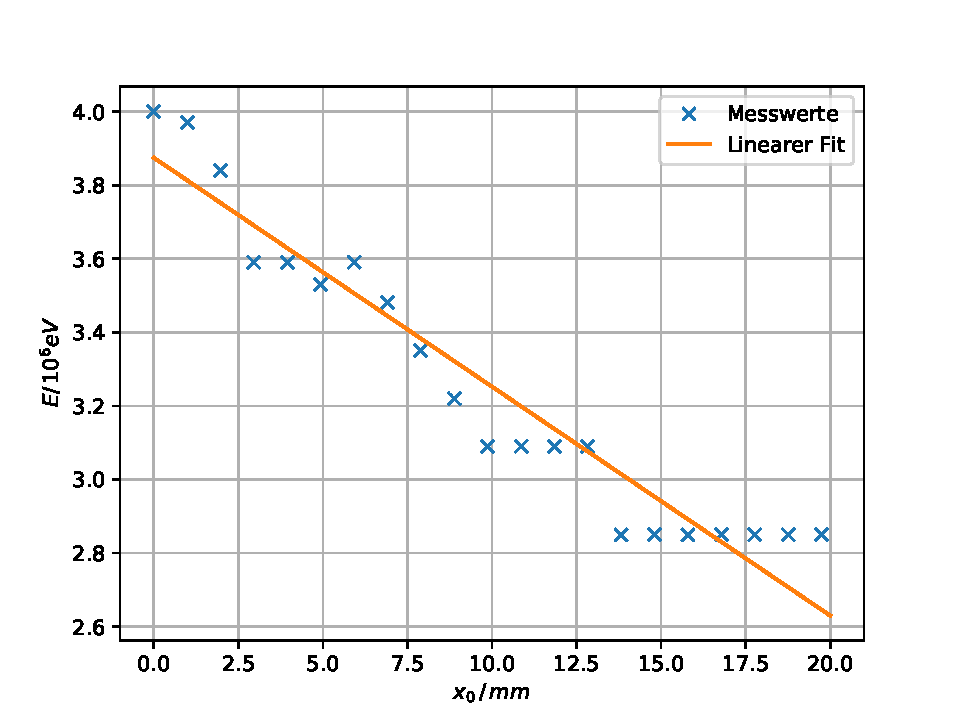
\includegraphics[width=0.8\linewidth]{energie_weglaenge2.pdf}
	\caption{Energie als Funktion der effektiven Länge $x_0$ für $l=2\,\symup{cm}$.}
	\label{fig:energie2}
\end{figure}

Der Energieverlust $-\frac{\symup{d}E}{\symup{d}x}$ ist jeweils der Betrag der Steigung der Ausgleichsgeraden, welche wiederum mit matplotlib erstellt werden.
Es werden folgende Werte ausgegeben:

\begin{equation*}
\begin{aligned}
-\frac{\symup{d}E}{\symup{d}x_{1{,}5}} &= (76{,}48 \pm 3{,}04)\,\symup{\frac{MeV}{m}} \\
-\frac{\symup{d}E}{\symup{d}x_2} &= (62{,}22 \pm 4{,}04)\,\symup{\frac{MeV}{m}} \\
\end{aligned}
\end{equation*}




\subsection{Statistik des radioaktiven Zerfalls}
In Tabelle \ref{tab:hundert} sind die Zählraten für hundert Messungen bei einem festen Abstand von $l = 2{,}5\,\symup{cm}$ zu finden.

\begin{table}[h!tbp]
\centering
\caption{Messwerte zur Bestimmung der Statistik.}
\label{tab:hundert}
\begin{tabular}{S[table-format=2] S[table-format=4] S[table-format=2] S[table-format=4] S[table-format=2] S[table-format=4]}
\toprule
{Messung} & {Zählrate} & {Messung} & {Zählrate} & {Messung} & {Zählrate}  \\
\midrule
1      & 7248 & 35 & 6576 &  69 & 6816 \\
2      & 6803 & 36 & 6673 &  70 & 7548 \\
3	   & 6875 & 37 & 6760 &  71 & 6675 \\
4	   & 7116 & 38 & 7170 &  72 & 7120 \\	   
5	   & 7116 & 39 & 7343 &  73 & 6950 \\
6	   & 7257 & 40 & 7356 &  74 & 7212 \\
7	   & 7132 & 41 & 6937 &  75 & 6912 \\
8	   & 7191 & 42 & 6837 &  76 & 6882 \\
9	   & 6716 & 43 & 6965 &  77 & 7030 \\
10	   & 6765 & 44 & 6886 &  78 & 6968 \\
11	   & 7085 & 45 & 6720 &  79 & 6678 \\
12	   & 6762 & 46 & 7017 &  80 & 7142 \\
13     & 7004 & 47 & 7042 &  81 & 6876 \\
14	   & 6572 & 48 & 6702 &  81 & 6876 \\
15	   & 6694 & 49 & 6821 &  82 & 7253 \\
16	   & 6888 & 50 & 7034 &  83 & 7120 \\
17	   & 6866 & 51 & 6876 &  84 & 6854 \\
18	   & 6596 & 52 & 6859 &  85 & 7255 \\
19	   & 7309 & 53 & 6729 &  86 & 7177 \\
20	   & 6851 & 54 & 6829 &  87 & 7277 \\
21	   & 6999 & 55 & 6687 &  88 & 7269 \\
22     & 6517 & 56 & 7078 &  89 & 6931 \\
23     & 7024 & 57 & 6676 &  90 & 6642 \\
24     & 6767 & 58 & 6791 &  91 & 6932 \\
25     & 6908 & 59 & 6777 &  92 & 7217 \\
26     & 6569 & 60 & 7005 & 93 & 7111 \\
27     & 6814 & 61 & 7516 & 94 & 6760 \\
28     & 6823 & 62 & 6942 & 95 & 7199 \\
29     & 7146 & 63 & 7025 & 96 & 6739 \\
30     & 6712 & 64 & 7022 & 97 & 7115\\
31     & 7048 & 65 & 6964 & 98 & 7046\\
32     & 7141 & 66 & 7022 & 99 & 7163\\
33     & 6879 & 67 & 7145 & 100 & 6661\\
34     & 7227 & 68 & 7381 & & \\
\bottomrule
\end{tabular}
\end{table}

Diese werden mit matplotlib in einem Histogramm aufgetragen. Ebenso wird mit dem Pythonmodul eine Gauß- und eine Poissonverteilung über die Messwerte gelegt, wie in Abbildung \ref{fig:histogramm} zu sehen ist.


\begin{figure}[h!]
	\centering
	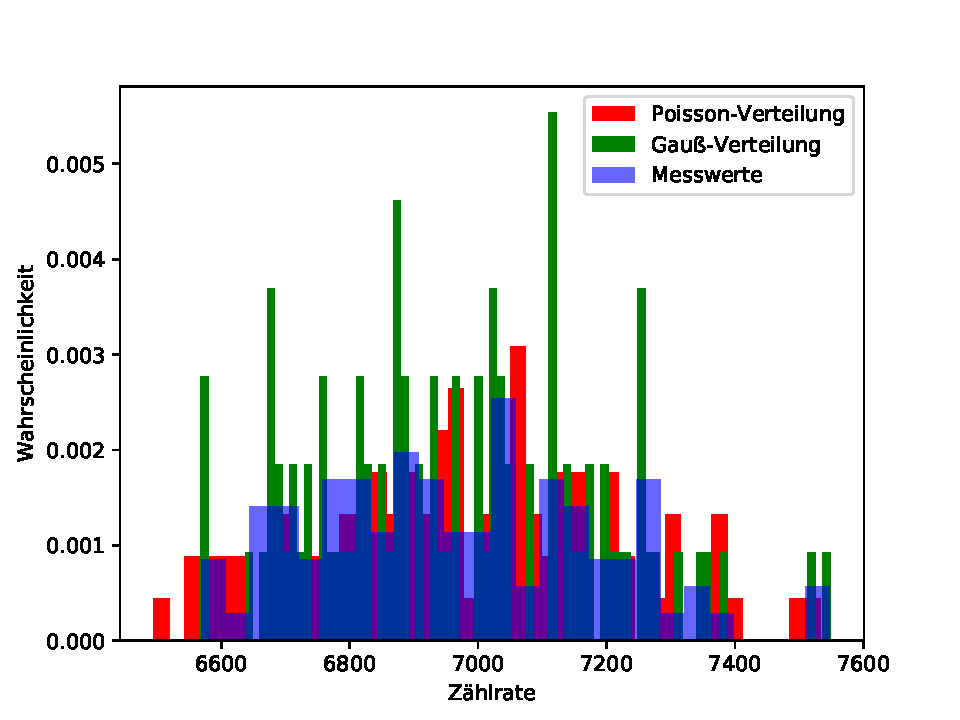
\includegraphics[width=1\linewidth]{test3.pdf}
	\caption{Histogramm der Messwerte, sowie Gauß- und Poissonverteilung.}
	\label{fig:histogramm}
\end{figure}



